\chapter{Überprüfung der Hypothese 1 \textit{\textcolor{gray}{(Autor: Subhan)}}}
\label{chap:hypothese1}

\section{Vorgehensweise}

\begin{enumerate}
    \item Für die deskriptive Analyse der Hypothese H1 werden wir bestimmte statistische Tests 
    durchführen, um zu überprüfen, ob die Hypothese mit den vorliegenden Daten angenommen oder 
    abgelehnt werden kann, wie unten in verschiedenen grafischen Darstellungen zusammen mit 
    relevanten Erklärungen und Ergebnissen dargestellt.
    \item Deskriptive Analyse Ist mit graphics abgedeckt
\end{enumerate}

Die unteren Tabelle \ref*{fig:h1_tabelle_alter} zeigen die durchschnittliche und die mittlere Meinung zu einer 4-Tage-Woche 
in verschiedenen Altersgruppen. Die durchschnittliche Meinung nimmt mit dem Alter leicht zu, 
während die mittlere Meinung für die jüngeren Altersgruppen (18-59 Jahre) konstant bei 1 oder 2 
bleibt und dann für die älteste Altersgruppe (60+ Jahre) auf 3,5 springt.

\begin{figure}[h]
    \centering
    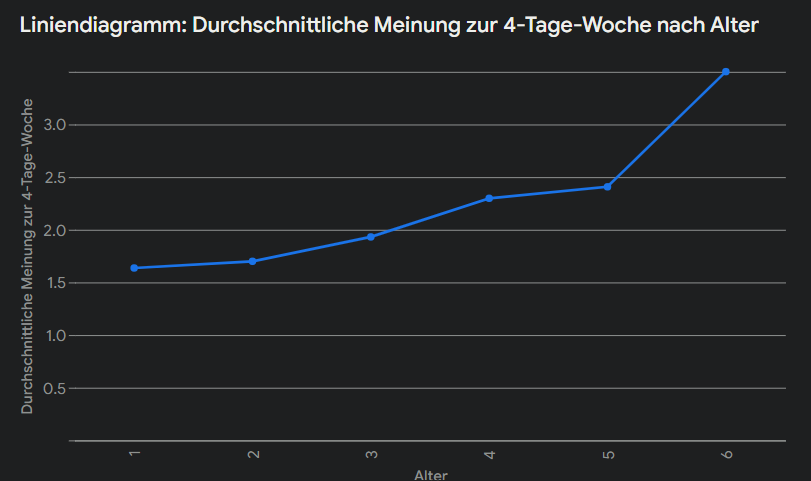
\includegraphics[width=0.8\textwidth]{04_Artefakte/01_Abbildungen/hypothese_1/h1_linie_alter.png}
     \caption{Meinung zu einer 4-Tage-Woche in verschiedenen Altersgruppen}
     \label{fig:h1_linie_alter}
\end{figure}

\begin{figure}[h]
    \centering
    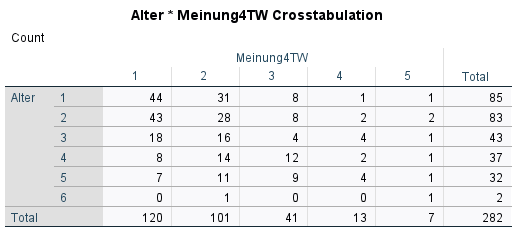
\includegraphics[width=0.8\textwidth]{04_Artefakte/01_Abbildungen/hypothese_1/h1_tabelle_alter.png}
    \caption{Häufigkeit der Meinungen zur 4-Tage-Woche in vers. Altersgruppen}
    \label{fig:h1_tabelle_alter}
\end{figure}

Die Kreuztabelle \ref*{fig:h1_tabelle_alter} bietet zusätzliche Einblicke in den Zusammenhang zwischen Alter und Meinung zur 
4-Tage-Woche und ergänzt damit die vorherige Analyse:

\textbf{Verteilung der Meinungen nach Altersgruppe:}

\begin{itemize}
    \item \textbf{Jüngere Altersgruppen (18-29 Jahre):}
    \begin{itemize}
        \item Überwiegend positive Meinungen (1, 2 auf der Skala)
        \item Wenige unentschiedene oder negative Meinungen (3, 4, 5)
    \end{itemize}
    \item Mittlere Altersgruppen (30-49 Jahre):
    \begin{itemize}
        \item Etwas gleichmäßigere Verteilung der Meinungen 
        \item Zunahme der positiven Meinungen (4, 5) im Vergleich zu den jüngsten Gruppen
    \end{itemize}
    \item \textbf{Ältere Altersgruppen (50+ Jahre):}
    \begin{itemize}
        \item Sehr kleine Stichprobengröße (insbesondere für Alter 6) 
        \item Tendenz zu eher positiven Meinungen, aber weniger ausgeprägt als bei den jüngeren.
    \end{itemize}
\end{itemize}

Beobachtungen in Bezug auf H1:

\begin{itemize}
    \item Die Hypothese, dass jüngere Menschen der 4-Tage-Woche positiver gegenüberstehen,
    wird teilweise unterstützt:
    \begin{itemize}
        \item Die Mehrheit der jüngsten Befragten (Alter 1 und 2) hat eine positive Meinung (1 oder 2).
        \item Allerdings gibt es auch in diesen Altersgruppen negative Meinungen.
    \end{itemize}
    \item Die Hypothese wird nicht durchgängig bestätigt, da positive Meinungen auch in den 
    älteren Altersgruppen vorhanden sind
\end{itemize}

Einschränkungen:
\begin{itemize}
    \item Die Stichprobengröße ist in den älteren Altersgruppen sehr gering, was die Aussagekraft der 
    Ergebnisse für diese Gruppen einschränkt.
\end{itemize}

\begin{figure}[h]
    \centering
    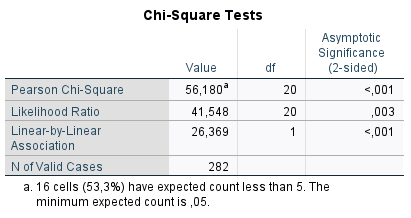
\includegraphics[width=0.8\textwidth]{04_Artefakte/01_Abbildungen/hypothese_1/h1_chi.png}
    \caption{Ergebnis des Chi-Quadrat-Tests für H4}
    \label{fig:h1_chi}
\end{figure}

Der in der Abbildung \ref*{fig:h1_chi} dargestellte Chi-Quadrat-Test wurde verwendet, um den Zusammenhang 
zwischen Alter und Meinung zur 4-Tage-Woche zu untersuchen, die für Hypothese H1 relevant ist.

Ergebnisse des Chi-Quadrat-Tests:
\begin{itemize}
    \item Pearson Chi-Square-Werte: 56.180
    \item Degrees of Freedom (df): 20
    \item Asymptotic Signifikanz (2-sided): p < .001
    \item Likelihood-Verhältnis: 41.548
    \item Linear-by-Linear Association: 26.369
\end{itemize}

\textbf{Interpretation:}
\begin{itemize}
    \item \textbf{Bedeutung des Zusammenhangs: }Die sehr niedrigen p-Werte (<.001 für Pearson und 
    Linear-by-Linear; .003 für Likelihood Ratio) weisen darauf hin, dass es einen statistisch 
    signifikanten Zusammenhang zwischen Alter und Meinung zur 4-Tage-Woche gibt. Das bedeutet, dass 
    die beobachteten Meinungsunterschiede zwischen den Altersgruppen wahrscheinlich nicht auf Zufall 
    beruhen.
    \item Stärke des Zusammenhangs: Der Chi-Quadrat-Test allein gibt keine Auskunft über die Stärke 
    des Zusammenhangs. Die vorherige Analyse mit der Korrelation (0.306) deutet jedoch auf einen 
    moderat positiven Zusammenhang hin.
    \item Linearität des Zusammenhangs: Der signifikante Linear-by-Linear Assoziationstest (p < .001) 
    deutet darauf hin, dass die Beziehung tendenziell linear ist, was bedeutet, dass mit abnehmendem 
    Alter die Zustimmung zur 4-Tage-Woche tendenziell zunimmt.
    \item Unterstützung der Hypothese H1: Die Ergebnisse des Chi-Quadrat-Tests stützen die Hypothese 
    H1 teilweise. Der signifikante Zusammenhang und die lineare Assoziation deuten darauf hin, dass 
    jüngere Menschen tendenziell positiver gegenüber der 4-Tage-Woche eingestellt sind als ältere 
    Menschen.
\end{itemize}

\begin{figure}[h]
    \centering
    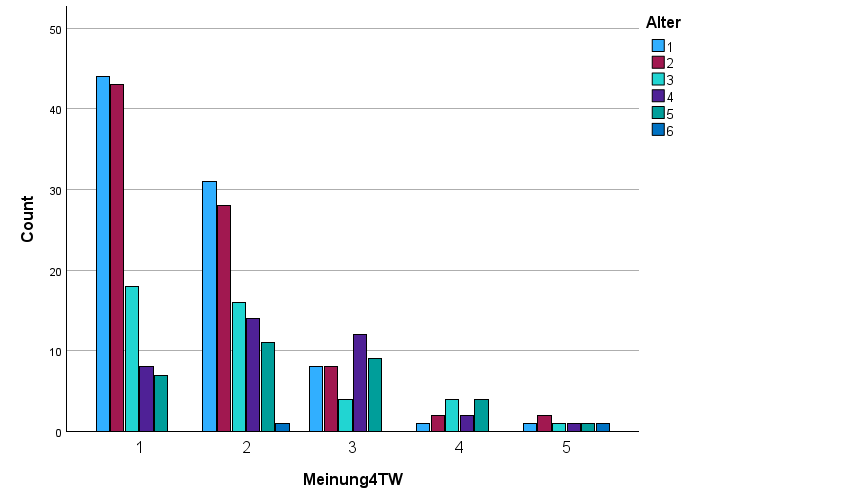
\includegraphics[width=0.8\textwidth]{04_Artefakte/01_Abbildungen/hypothese_1/h1_graph.png}
    \caption{Interpretation der Allgemeine Trend in Vers. Alter Gruppen}
    \label{fig:h1_graph}
\end{figure}

Der Graph \ref{fig:h1_graph} veranschaulicht die Verteilung der Antworten auf die Frage \gqq{Meinung4TW}
(Meinung zur 4-Tage-Woche) über verschiedene Altersgruppen (\gqq{Alter}). Dies ist direkt relevant für 
die Hypothese H1, die besagt, dass jüngere Menschen eher eine positive Meinung zur 4-Tage-Woche haben.


\textbf{Interpretation des Diagramms \ref{fig:h1_graph} in Bezug auf H1:}
\begin{itemize}
    \item \textbf{Allgemeiner Trend:  }Es scheint einen allgemeinen Trend zu geben, der H1 unterstützt. 
    Die jüngeren Altersgruppen (1 und 2) haben höhere Anzahlen bei den niedrigeren Meinung4TW-Werten 
    (1 und 2), was auf eine positivere Meinung zur 4-Tage-Woche hinweist.
    \item \textbf{Nuancen: }Der Trend ist nicht perfekt linear. Während die jüngste Gruppe (1) die stärkste 
    Präferenz für die positivste Meinung (1) zeigt, zeigen auch die mittleren Altersgruppen (3 und 4) 
    eine beträchtliche Anzahl positiver Antworten. Die ältesten Gruppen (5 und 6) haben insgesamt weniger 
    Antworten, was es schwieriger macht, eindeutige Schlussfolgerungen zu ziehen.
\end{itemize}

\textbf{Einschränkungen:}
\begin{itemize}
    \item \textbf{Stichprobengröße:  }Die Stichprobengröße für die älteren Altersgruppen ist gering, 
    was die Verallgemeinerbarkeit der Ergebnisse für diese Gruppen einschränkt.
    \item \textbf{Meinungsskala: }Das Diagramm zeigt nur die Verteilung der Meinungen, nicht die 
    Intensität dieser Meinungen. Jemand, der \gqq{2} wählt, könnte nur leicht positiv eingestellt sein, 
    während jemand, der \gqq{1} wählt, sehr begeistert sein könnte. Diese Nuance geht in dieser 
    Visualisierung verloren.
\end{itemize}

\textbf{Allgemein:}
Der Graph liefert visuelle Belege, die H1 teilweise stützen. Jüngere Menschen neigen zwar dazu, 
positivere Meinungen zur 4-Tage-Woche (4TW) zu haben, aber der Trend ist nicht so eindeutig, wie 
die Hypothese nahelegt. Ältere Altersgruppen haben immer noch eine beträchtliche Anzahl positiver 
Meinungen, und die geringe Stichprobengröße für die ältesten Gruppen macht es schwierig, endgültige 
Schlussfolgerungen über ihre Ansichten zu ziehen.

\begin{figure}[h]
    \centering
    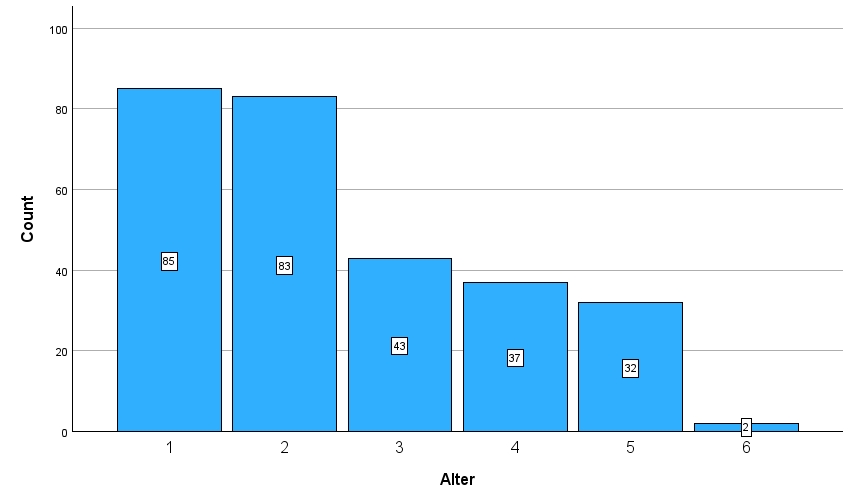
\includegraphics[width=0.8\textwidth]{04_Artefakte/01_Abbildungen/hypothese_1/h1_saeulen.png}
    \caption{Verteilung der Befragten über verschiedene Altersgruppen in den Umfragedaten}
    \label{fig:h1_saeulen}
\end{figure}

Das Balkendiagramm \ref*{fig:h1_saeulen} veranschaulicht die Verteilung der Befragten über verschiedene Altersgruppen in den 
Umfragedaten. Es steht in direktem Zusammenhang mit der Hypothese H1.

\section{Beobachtungen:}

\textbf{Verteilung der Altersgruppen:}
\begin{itemize}
    \item Die Mehrheit der Befragten gehört den jüngeren Altersgruppen an (1, 2 und 3).
    \item Mit zunehmendem Alter nimmt die Anzahl der Befragten spürbar ab.
\end{itemize}

\begin{itemize}
    \item \textbf{Stichprobengröße:}
    \begin{itemize}
        \item Die Stichprobengröße für ältere Altersgruppen (5 und insbesondere 6) ist recht klein
    \end{itemize}
\end{itemize}

\textbf{Implikationen für H1:}
\begin{itemize}
    \item Begrenzte Repräsentativität älterer Befragten: Die geringe Stichprobengröße für ältere 
    Altersgruppen erschwert es, endgültige Schlussfolgerungen über ihre Ansichten zur 4-Tage-Woche zu 
    ziehen. Dies schränkt die Möglichkeit ein, die Hypothese für das gesamte Altersspektrum vollständig 
    zu testen.
    \item Potenzial für Bias: Die Überrepräsentation jüngerer Befragter könnte die Analyse verzerren, 
    da ihre Ansichten möglicherweise nicht repräsentativ für die gesamte Bevölkerung sind.
\end{itemize}

\section{Prüfung der Hypothesis}
Die Hypothese H1, die besagt, dass jüngere Menschen eine positivere Meinung zur 4-Tage-Woche hätten, 
wird durch die Daten nicht stark unterstützt. Zwar nimmt die durchschnittliche Zustimmung mit dem Alter 
leicht zu, der Median der Meinungen bleibt jedoch in den jüngeren Altersgruppen relativ konstant. Der 
größte Unterschied zeigt sich in der ältesten Altersgruppe (60+ Jahre), die eine deutlich weniger 
positive Meinung aufweist.

